\section{Evidences of Learning with the Integrator Project}
\label{sec:gralIntegratorProject}
Figure~\ref{fig:evidenceDistribution} details each evidence with the estimated 
time inside and outside the classroom. There are several kinds of activities in the 
initial and final explanation of the integrator project like practices 
and exams. Next sections explain in detail such an evidences.
\begin{figure}[hbt]
 %\begin{center}
  \centering
    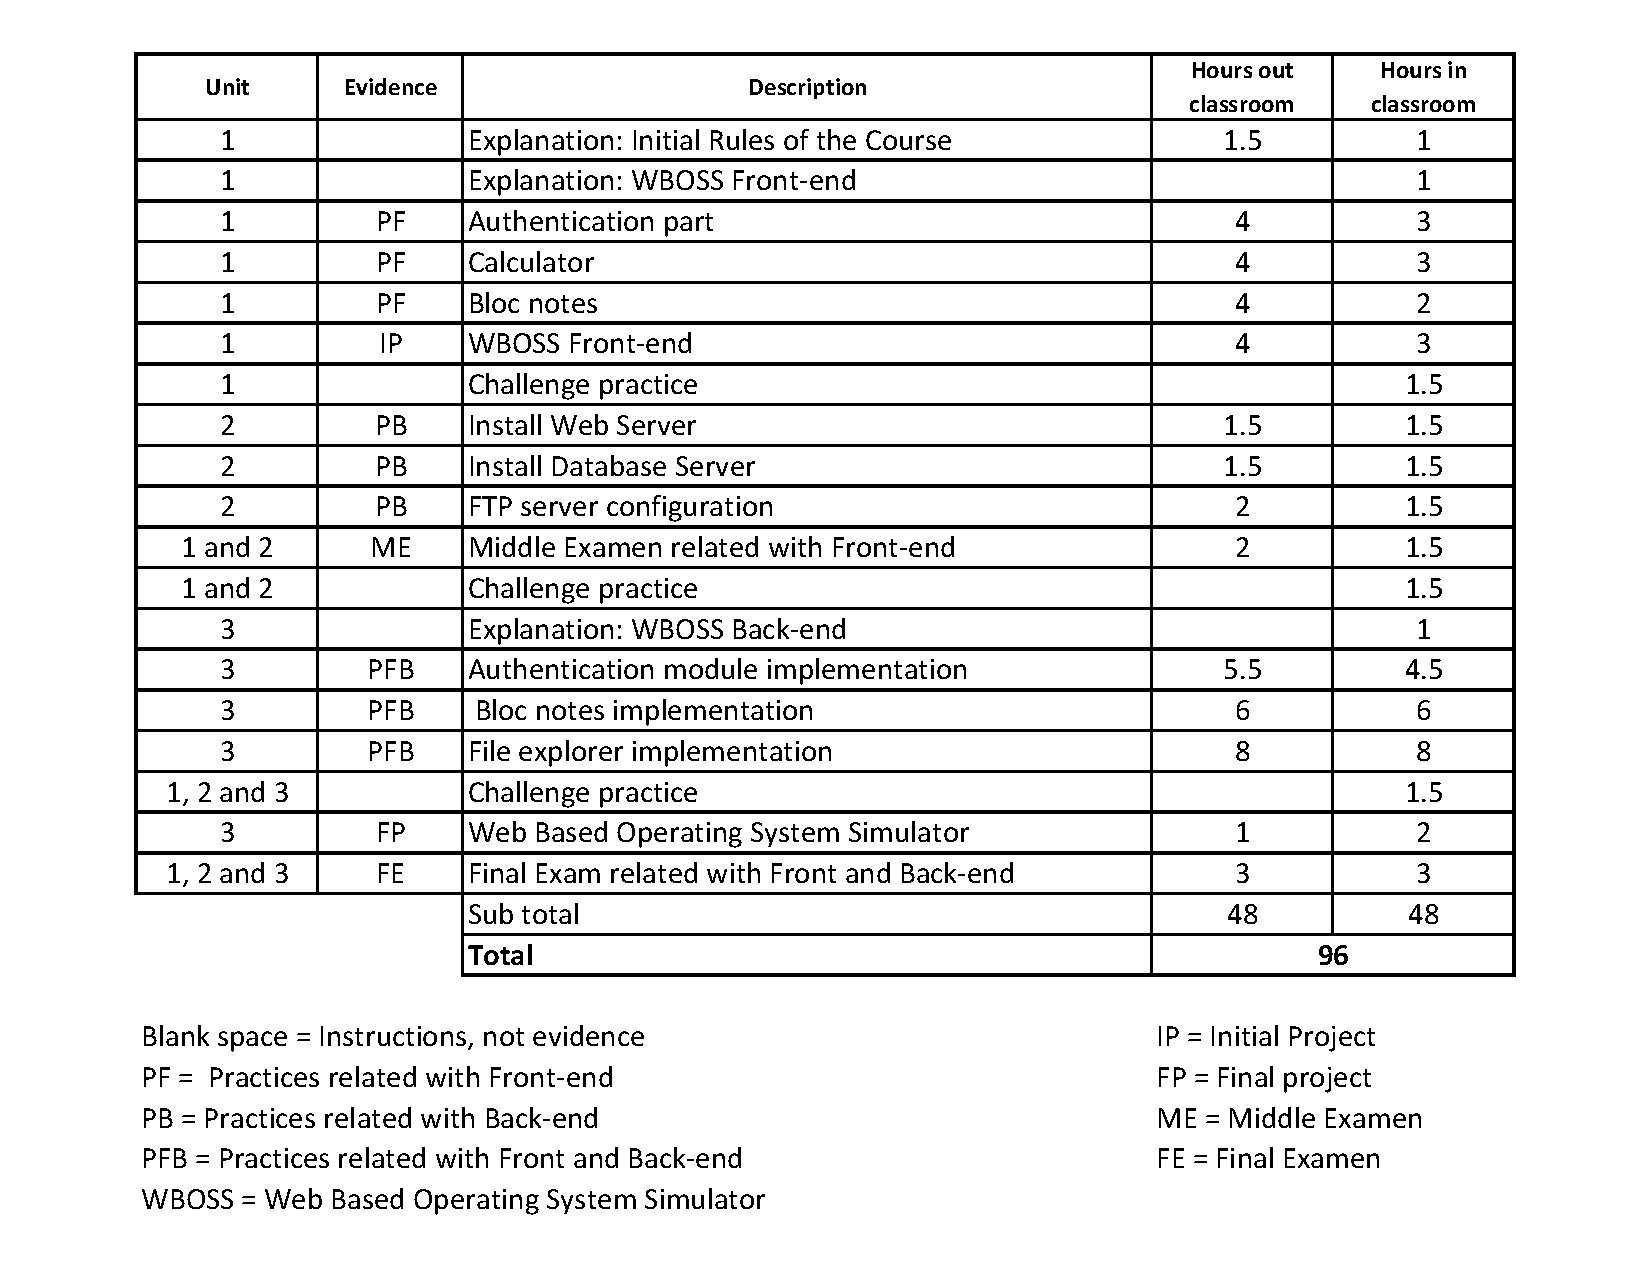
\includegraphics[scale=0.5]{images/evidenceDistribution.pdf}
        \caption{Detail of all evidences applied in the course of web programming }
    \label{fig:evidenceDistribution}
 % \end{center}
\end{figure}

%\subsection{Integrator Project}
\subsection{Integrator Project}
\label{ssec:integratorProject}
The integrator project is explained to the students in two stages: 
at the beginning and in the middle of the course. 
In both stages are explained the scopes and the deadline.

\subsubsection{Initial project: Design of the Simulator}
\label{sssec:desginOS}
With the development of the initial project students will achieve their learning in 
topics like HTML, CSS, JavaScript and derived libraries (Unit 1, Section~\ref{ssec:learningUnits}). 
In this stage, high design content is requested, especially because it seeks to get students to stick as 
closely as possible to the design of the simulated OS, that is where students 
confirm the use and learning of CSS. 
Some students may download images that are very similar 
to the selected OS, this is valid because they learn to 
manipulate the use and positioning of images.

The initial project specification together with the knowledge the students must acquire or apply is shown 
in Table~\ref{table:initialProject}.
%If the selected OS does not cover the aforementioned aspects, students must invent it 
%or do something additional to comply with the specified points.

\begin{table}[htb]
    \begin{center}
        \caption{Initial project content. Learning topics: H=HTML, C=CSS, J=JavaScript, D=DOM, Q=JQuery}
        \label{table:initialProject}
        \begin{tabular}{|l|l|l|l|l|l|l|l|}
        \hline
Activity&  Description                                      & H     & C     & J     & D     & Q   \\\hline

Identity& Show in some ingenious section personal data of   &$\surd$&$\surd$&       &       &     \\
        & the developer and information of the subject      &       &       &       &       &     \\
        & (including at least a figure).                    &       &       &       &       &     \\\hline

Login   & Show at the beginning of the OS an authentication &$\surd$&$\surd$&       &       &     \\
        & mechanism. Post method is not required yet.       &       &       &       &       &     \\\hline
        
Desktop & Show the startup desktop. This faces several      &$\surd$&$\surd$&       &       &     \\
        & design challenges considering different existing  &       &       &       &       &     \\
        & Operating Systems.                                &       &       &       &       &     \\\hline

Options & All OS's have a main menu which let to navigate   &$\surd$&$\surd$&       &       &     \\
        & for different options. The simulator must contain &       &       &       &       &     \\
        & at least the following options: Identity,         &       &       &       &       &     \\
        & Calculator and Notes.                             &       &       &       &       &     \\\hline

Calculator& Show a calculator with a very similar appearance&$\surd$&$\surd$&$\surd$&       &     \\
        & with the design of the selected Operating System. &       &       &       &       &     \\
        & It must calculate arithmetic operations such as   &       &       &       &       &     \\
        & addition, subtraction, multiplication, division   &       &       &       &       &     \\
        & and residual (mod).                               &       &       &       &       &     \\\hline

Notes   & Show a system able to create and delete notes.    &$\surd$&$\surd$&$\surd$&$\surd$&$\surd$\\
        & Data persistence is not requested yet.            &       &       &       &       &     \\\hline
        \end{tabular}
    \end{center}
\end{table}


%\begin{itemize}
%    \item \textbf{Login:} show at the beginning of the OS an authentication mechanism. 
%        Students must apply knowledge in HTML, CSS and Forms. Although not knowing yet
%        how to use the GET and POST methods.
%    \item \textbf{The desktop:} show the startup desktop. This faces several design 
%        challenges considering 
%        the different proposals that exist in Operating Systems. Students must apply 
%        high knowledge of HTML and CSS.
%    \item \textbf{Options:} all OS's have a main menu letting to navigate, the simulator
%        must contain at least the following:
%        Identity, Calculator; and Notes.
%    \item \textbf{Identity:} it must be placed in some ingenious section of the selected 
%        Operating System and must show the personal data of the developer of the page, 
%        the logo of the university, the subject, and the name of the teacher.
%    \item \textbf{Calculator:} when clicking on this option, a calculator must be displayed
%        similar in design to the chosen Operating System, and it must calculate arithmetic 
%        operations such as addition, subtraction, multiplication, division and residual (mod). 
%        This involves consolidating knowledge in JavaScript, HTML and CSS.
%    \item \textbf{Notes:} When clicking on this option, a system of notes (create and delete 
%        notes) should appear. As it has not yet seen the issues that involve the server is 
%        not requested data persistence. This section allows the student to consolidate their 
%        knowledge between JavaScript and their access to the HTML DOM, either by JavaScript 
%        primitives or by JQuery.
%\end{itemize}


\subsubsection{Final Project: Operating System Simulator}
\label{sssec:finalProyDesc}
The final project description is explained after the students have carried out 
the practices with the installation of different servers; and once the client/server 
concepts have been explained. 
Students may propose which Server programming language are going to work with. 
It is important that each student makes a decision in advance. 
With this, we achieve that each student has a different operating system to design and
to develop; and maybe, with a different programming language of their own preference.
This stage consists of continuing the initial project 
and extending it as explained in Table~\ref{table:lastPartProject}.
\begin{table}[htb]
    \begin{center}
        \caption{Second part of the project. Server's Learning topics: S=Server Programming, D=Database, F=Files, A=AJAX, I= Improve Front-End}
        \label{table:lastPartProject}
        \begin{tabular}{|l|l|l|l|l|l|l|l|}
        \hline
Activity&  Description                                      & S     & D     & F     & A     & I   \\\hline

Login   & Use of database and JavaScript validations.       &$\surd$&$\surd$&       &       &     \\
        & Implementation, at least, two different user      &       &       &       &       &     \\
        & profiles: a) Administrator and b) Normal user.    &       &       &       &       &     \\\hline
        
Options & According to the user profile, the Aministrator   &$\surd$&$\surd$&       &       &$\surd$\\
        & can add other users; while the normal user can    &       &       &       &       &     \\
        & navigate between the different options (see       &       &       &       &       &     \\
        &Table~\ref{table:initialProject}) and extended here.&       &       &       &       &     \\\hline

Users   & The administrator can add, delete, update and list&$\surd$&$\surd$&       &       &$\surd$\\
Manager & other users. Each user can update his own data.   &       &       &       &       &     \\\hline

Text   & Extend the Notes system of 
             Table~\ref{table:initialProject}, now the user &$\surd$&$\surd$&$\surd$&$\surd$&$\surd$\\
Editor  & can add, delete, update and list his own notes.   &       &       &       &       &     \\
        & Data persistence is required. It must contain at  &       &       &       &       &     \\
        & least the following characteristics: font family  &       &       &       &       &     \\
        & font size, "do" and "undo" options.               &       &       &       &       &     \\\hline

File    & Create new plain-text files, delete it or rename  &$\surd$&$\surd$&$\surd$&$\surd$&$\surd$\\
Explorer& it. The files must be created on the web server.  &       &       &       &       &     \\\hline  
        \end{tabular}
    \end{center}
\end{table}

%\begin{itemize}
%    \item Server-side programming language: students may propose one of their own interest
%        or one learned in class. 
%        It is important that each student makes a decision in advance. 
%        With this, we achieve that each student has a different operating system to design and
%        to develop; and maybe, with a different programming language of their own preference.
%    \item Loguin implementation: use of database and validations with JavaScript or HTML5. 
%        At least, two different user profiles must be considered: a) Administrator and b) Normal user.
%        The administrator can add other users; while
%        the normal user can navigate between the different options explained in the initial part of 
%        the project and extended below.
%    \item Persistence of data: implement the use of CRUD\footnote{Operations Create, Read, 
%        Update and Delete} operations in databases. It consists in extending the \textbf{Notes},
%        where the user could add, delete, update and list his own notes.
%    \item Files: text editor with some capabilities (at least, change source, 
%        change font size, "do" and "undo" options, save plain-text files, and update it.
%    \item File Explorer: create new plain-text files, delete it or rename it. The 
%        files must be created on the web server.
%\end{itemize}


\subsection{Practices}
Sometimes it is usual for students to share the solutions of their jobs and even more when they 
are the same between different generations. To avoid this, we recommend to divide the Simulator 
into small practices. 
It is inevitable that sometimes students can share code for some solutions, however this is not 
so relevant, because it also encourages the reuse of code; it is important that students know 
how to adapt the code of another solution to their own solutions. 
So we break up all practices in three groups: Front-end, Back-end and Client-Server interaction.

\subsubsection{Front-end}
Practices focused on supporting the development of the simulator but also on clarifying topics 
such as HTML, CSS (respectively HTML5 and CSS3) and JavaScript. 
Table~\ref{table:initialProject} describes, in general, each practice. 
Next, we explain it in detail:
\begin{itemize}
    \item HTML (first practice): design an \textbf{Identity} html page. 
        With this the students must learn: 
        i) The general structure of an html page;
        ii) Basic tags to format fonts;
        iii) Understand about the correct structure of a web page; and
        iv) Understand that HTML and CSS are not programming languages.
        \footnote{See an example of this practice at \url{\pathpractices client01.pdf}}
    \item HTML and CSS (second practice): Design a \textbf{Login}:
        i) they can use (among other things) the use of divs, inputs, forms, links; and
        ii) they can start using CSS. Post and Get methods are not necessary to know yet.
        \footnote{See an example of this practice at \url{\pathpractices client02.pdf}}
    \item HTML, CSS and JavaScript (third practice): Design a calculator. With this practice the 
        students:
        i) understand the different ways to include styles to a web page (Use of CSS);
        ii) know the use of CSS selectors, the use of ids and class;
        iii) execute a simple JavaScript code;
        iv) know how to call functions from events in html tags (i.e. \textit{onclick});
        v) use logical and arithmetic operators in JavaScript;
        \footnote{See an example of this practice at \url{\pathpractices client03.pdf}}
    \item HTML DOM, Frameworks Front-end and JavaScript libraries (fourth practice): 
        Design a light version of a note system. Students must learn how to:
        i) Position, size colors, etc. to the blocks and text labels;
        ii) Access the DOM through JavaScript;
        iii) Perform different operations between JavaScript and the HTML DOM.
        In this part, students may apply some Front-end frameworks like Bootstrap, JQuery,
        etc.
        \footnote{See an example of this practice at \url{\pathpractices client04.pdf}}
\end{itemize}

In each of the above practices, students may include more tags than required, 
but it is important to emphasize that they must understand all tags 
included in their practices. A good suggestion is to do the review of the different 
activities in plenary and to make feedback with other tags used by other students,
with this, students learn also from their classmates. 

In addition, each of the practices must be related with the selected operating system. 
Although we suggest not to evaluate the design yet, it is better to wait until 
they have the first delivery of the Initial project because students could acquire 
more design skills.

\subsubsection{Back-end}
Nowadays to configure web working tools for developers using technologies such as LAMP, XAMP, WAMP 
and MAMP is relatively easy. 
However, installing one of these technologies causes to ignore servers concepts configuration
such as the Web Server, Database Management System (DBMS), FTP server; besides forgetting important 
aspects such as configuration about the ip, port number, id of the session, maximum amount 
of file upload, etc., which are part of the web paradigm. For this reason, we propose:
\begin{itemize}
    \item Install a Web Server: deliver a practice with code 
        executing in the server side and another executing in the client side.\footnote{See 
            an example of this practice at \url{\pathpractices server01.pdf}} 
        It is not requested a particular Web Server, because an objective is that students 
        might explore different technologies. Something important is to know the main
        configurations to upload the files that will be processed by the server. 
    \item Client vs Server side: comprehend which part of the script runs 
        on the server and which part on the client. To do that, students must deliver a practice 
        very similar with the first one, but now they must deliver it in two different 
        computers: one being the web server and the other one using the browser.\footnote{See an
            example of this practice at \url{\pathpractices server02.pdf}}
    \item Install a DBMS: understand the APIs required to establish communication between the web server, 
        and the database server. \footnote{See an example of this practice at \url{\pathpractices server03.pdf}}
\end{itemize}

We have identified that some students without background in Network topics
have some difficulties to understand quickly Client and Server processing.
We recommend this topic previously to a Web Programming course.

\subsubsection{Client-Server interaction}
%These practices are focused to understand programming on the Client and the Server side. 
In these practices the student must already have knowledge about Front and Back End. 
He must be prepared to incorporate a mixture of technologies to close with his integrator 
project. We propose to work in the second part of the simulator project in various practices
explained as follows:
\begin{itemize}
    \item Cookies and database connection: implement a simple authentication mechanisms 
        (See Login in Table~\ref{table:lastPartProject}) by 
        accessing to a database and to decide what type of user has been initiated (a simple 
        version as suggested by Francesco Maiorana~\cite{Maiorana14}). In this practice, the 
        students intensify their knowledge with respect to different instructions of programming 
        in the server side. They also improve their level of learning on the client side 
        (JavaScript), by means avoiding data latency doing some validations in the client 
        side. It is suggested to apply cookie concepts.
        \footnote{See an example of this practice at \url{\pathpractices clientServer01.pdf}}
    \item CRUD operations in DBMS: implement the User Manager system of  
        Table~\ref{table:lastPartProject} where it is possible to 
        add, delete, update and list users personal data.
    \item Files and Session variables: implement a block of notes system where each user
        can create, read, update, and his own files. Files must be created in the server
        side.
        \footnote{See an example of this practice at \url{\pathpractices clientServer02.pdf}}
    \item AJAX: implement the File explorer of  
        Table~\ref{table:lastPartProject}
        where each user can list and delete his own files in real time. It must be possible to open the listed
        files with the Block of Notes, it must contain a file searcher using asynchronous communication, 
        in other words, while the user type a key its file coincidences should be appearing.
        \footnote{See an example of this practice at \url{\pathpractices clientServer03.pdf}}
\end{itemize}


\subsection{Knowledge}
Within Competency-Based Assessment, knowledge is a competence that students must acquire during 
a course. According to the first two levels of Bloom's cognitive domain~\cite{BloomTaxonomy2001}, 
knowledge and understanding are basic and very important skills that a student must possess, 
since the learned concepts serve to relate new knowledge.

One of the instruments used to identify, in students, the competence of knowledge is to perform a 
test, which can be theoretical and/or practical. 
The theoretical tests usually measure knowledge, and it is an evidence if the student learned the concepts, 
but at no time do you know if he acquired the skills to solve certain problems.
Usually practical tests give you evidence that the student has acquired some skills. The problem of 
its application is to know if the given time to the students to solve a test is appropriate, since 
some may finish faster than others.  Table~\ref{table:learningEvidences} emphasizes the percentage we 
evaluate with skills by 65\% and knowledge by 35\%.


Regardless of the type of test applied to the student, it also serves to identify possible weaknesses 
that the students contain and then work with them to reinforce them. Hence, two exams are proposed: 
midterm and final.

The midterm exam is split in two parts:
i) concepts;\footnote{See an example of this at \url{\pathexams midTermConceptExam.pdf}} and 
ii) a small problem.\footnote{See an example of this at \url{\pathexams midTermProblemExam.pdf}} 
The concepts is in order to know general and basic aspects about understanding Front-end terms. 
It is not about students memorizing the use of HTML tags, CSS attributes or JavaScript instructions 
but they must know some basic aspects. The second part consists in solving a small problem through 
JavaScript language and HTML DOM.

On the other hand the final exam is also split in two parts: 
i) concepts; \footnote{See an example of this at \url{\pathexams finalConceptExam.pdf}} and 
ii) a small problem.\footnote{See an example of this at \url{\pathexams finalConceptExam.pdf}} 
The concepts have the objective that students demonstrate understanding on the Client/Server 
architecture, HTTP protocol, configuration ports, session variables, cookies and AJAX. 
The problem part consists in solving a small problem using server programming.
